\chapter{Results}
\label{chap:Results}

Below is the path followed by a randomly selected particle with initial energy $E=10^{14}$eV:

\begin{figure}[H]
    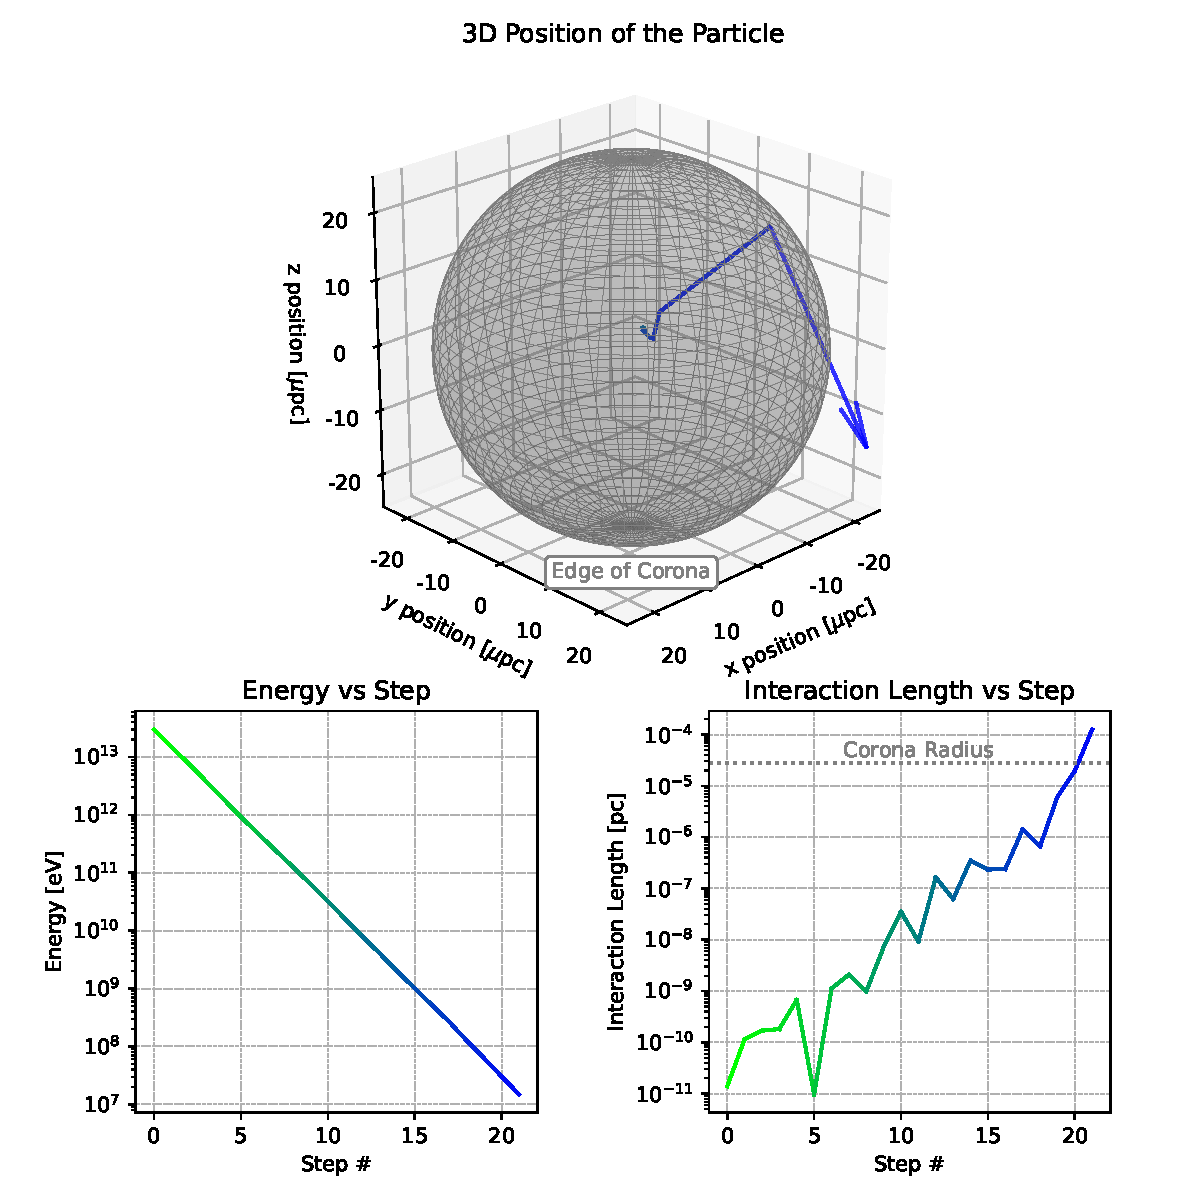
\includegraphics[width=0.88\textwidth]{Figures/example_random_walk.pdf}
    \centering
    \caption{Parameters of the 3D random walk of a random particle $(\theta_{\max}=\pi)$. The blue arrow indicates the last position is outside the graph in said direction. Also represented are the energy of the particle in each step and the interaction length of every step. When this last one becomes bigger than $R_c$, the particle escapes.}
    \label{fig:example_random_walk}
\end{figure}

As it can be seen, the energy of the particle gets reduced exponentially in every collision. We would expect it to be close to $E_\text{final} = E_\text{initial}\cdot 0.5^{\#_\text{coll.}}$. Now, after binning the particles according to their energy, we can represent the simulated flux:

\begin{figure}[H]
    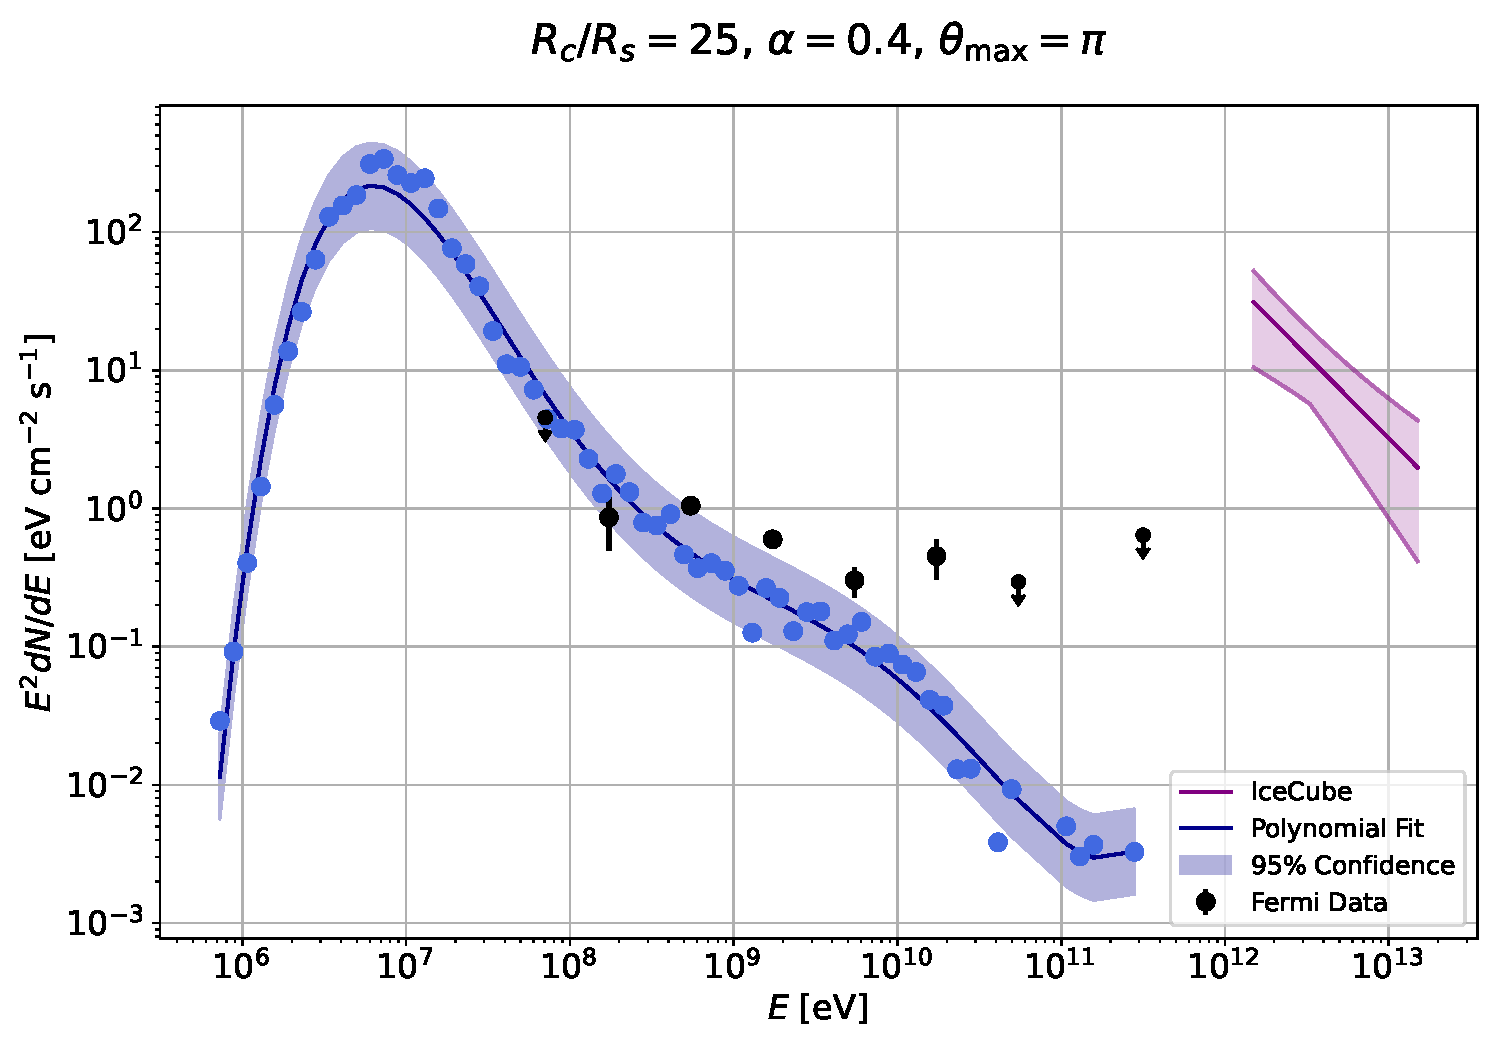
\includegraphics[width=\textwidth]{Figures/example_simulation_plot.pdf}
    \centering
    \caption{Spectral Energy Distribution of NGC1068's AGN for $R_c=25R_s$, $\alpha=0.4$ and $\theta_{\max} = \pi$. The blue line represents the 10-year data from IceCube, as well as our initial flux for the photons. The red dots are the simulated flux from the model. A polynomial of degree 5 has been fitted into the data. The 95\% confidence interval is also represented. Finally, the 4-year data from Fermi is represented as the black dots and upper limits.}
    \label{fig:example_simulation_plot}
\end{figure}

These are the results of the simulation for said values of the coronal radius, alpha and the turning angle, which are within reasonable expectation of the real values.

However, it is also of great interest to check what the results of the model are for other values of the corona. This way, we can check whether there is a combination of these parameters which fits more accordingly the data from Fermi. Doing so, produces the following series of plots:

\begin{figure}[H]
    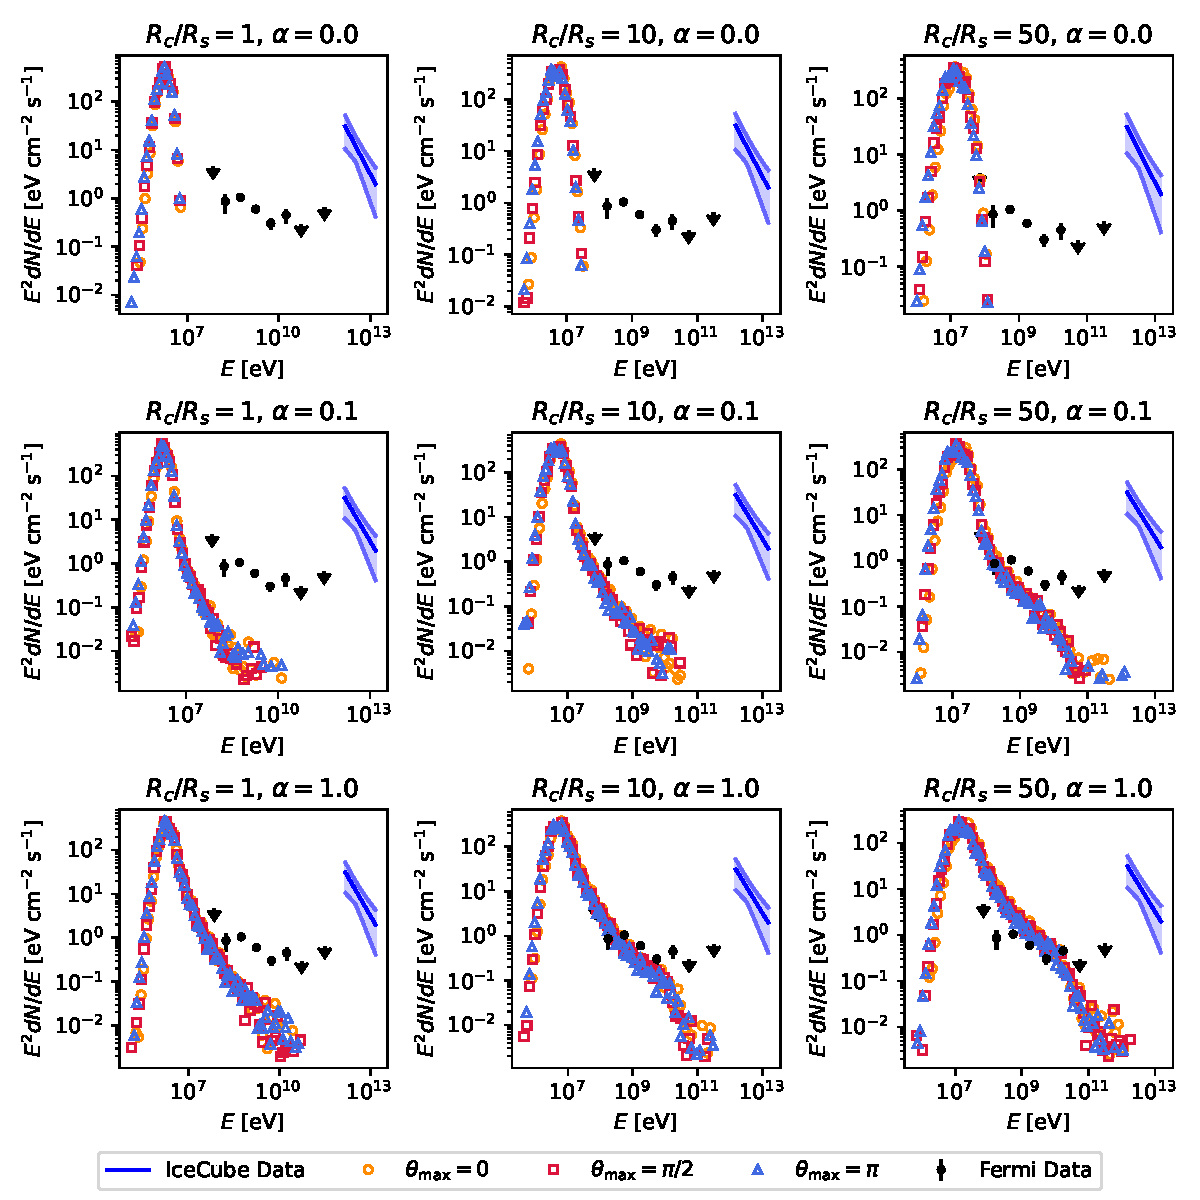
\includegraphics[width=\textwidth]{Figures/simulations_plot.pdf}
    \centering
    \caption{Spectral Energy Distribution of NGC1068's AGN for different values of $Rc$, $\alpha$ and $\theta_{\max}$. The blue line represents again the data from IceCube and our initial flux for the photons. The red, blue and yellow symbols represent the flux for different values of $\theta_{\max}$. The 4-year data from Fermi is represented as the black dots and upper limits.}
    \label{fig:simulations}
\end{figure}

One interesting thing one can take away from this plot is $\theta_{\max}$ has very little influence in the results. Beamed particles tend to have slightly higher energies due to the fact that they're prone to taking less steps when cascading. However, there is practically no difference between the particles executing a complete random walk and being beamed.

This means that the interaction length of the photons is the quantity which dictates the final spectral energy distribution of the system. 

These simulations are quite resource and time intensive. In order to find which parameters yield a better fit for the IceCube data, it is not practical to run the simulation for every possible combination of the parameters. Instead, we can use a machine learning algorithm to find the best fit.

The objective is to predict which shape the spectrum will have given a certain combination of the coronal radius and $\alpha$ \footnote{Since the maximum turning angle's effect has been shown to be negligible, I will simply assume the spectrum depends on said two parameters.}. In order to do this, I initially feed the machine learning algorithm the simulated spectra for different values of $R_c$ and $\alpha$. It then learns the patterns which emerge from these spectra and creates a prediction for what shape it will have.

% In this chapter, you describe the output from applying your methodology. Present your results in a clear manner, using a combination of figures and tables.

% If you are doing lab experiments: What do you observe? Also include qualitative observations that might not be directly relevant (“we saw more production at the upper half of the core sample than the lower half, with most production leaving at the upper side-plane”).

% If you are doing computations: What is the output from applying your code/software? Which part of your software is using the most computational power? How does it compare to other similar software?

% Illustrate the results. Use graphs, images, and tables (see Chapter \ref{chap:Theory}).

% A common challenge is to distinguish the results and the discussion section. Do not discuss your results in this chapter, that should be done in the discussion section. If it is hard to separate results and discussion, you might combine them into one section. You could also split the results and discussion part of your thesis into several results/discussion sections for different topics (“Magnesium effect on imbibition”, “Sodium effect on imbibition”).

% Try to avoid repetition between. In case you have many graphs of the same process, keep some characteristic graphs and move the rest to an appendix. Then you describe one graph in detail and refer to the others in the appendix for changes between the results.